Primero extendimos el pliego sobre la mesa y trazamos con grafito una línea horizontal larga, que fue nuestro eje $x$ y a la vez nuestro espejo. Del lado derecho marcamos un punto O que tomamos como origen, y por él pasamos una línea perpendicular.

Después vinieron los puntos.

Arriba del espejo colocamos el punto A a la izquierda y el punto B a la derecha, ambos a una distancia considerable de la línea. Para obtener la imagen A' bajamos desde A una perpendicular al espejo y la prolongamos del otro lado la misma distancia que había entre A y la línea, exactamente como se vería A dentro de un espejo real.

Sobre el espejo elegimos siete puntos, de P1 a P7. No los pusimos igualmente espaciados; algunos quedaron juntos cerca de donde sospechábamos que estaría el mínimo y otros más lejos, mientras que P7 quedó justo en el origen O. Luego, con un color diferente para cada uno, unimos A con cada punto P y cada punto P con B, y también trazamos la línea de A' hacia cada P, como se ve en la figura \ref{fig:trazo}.

\begin{center}
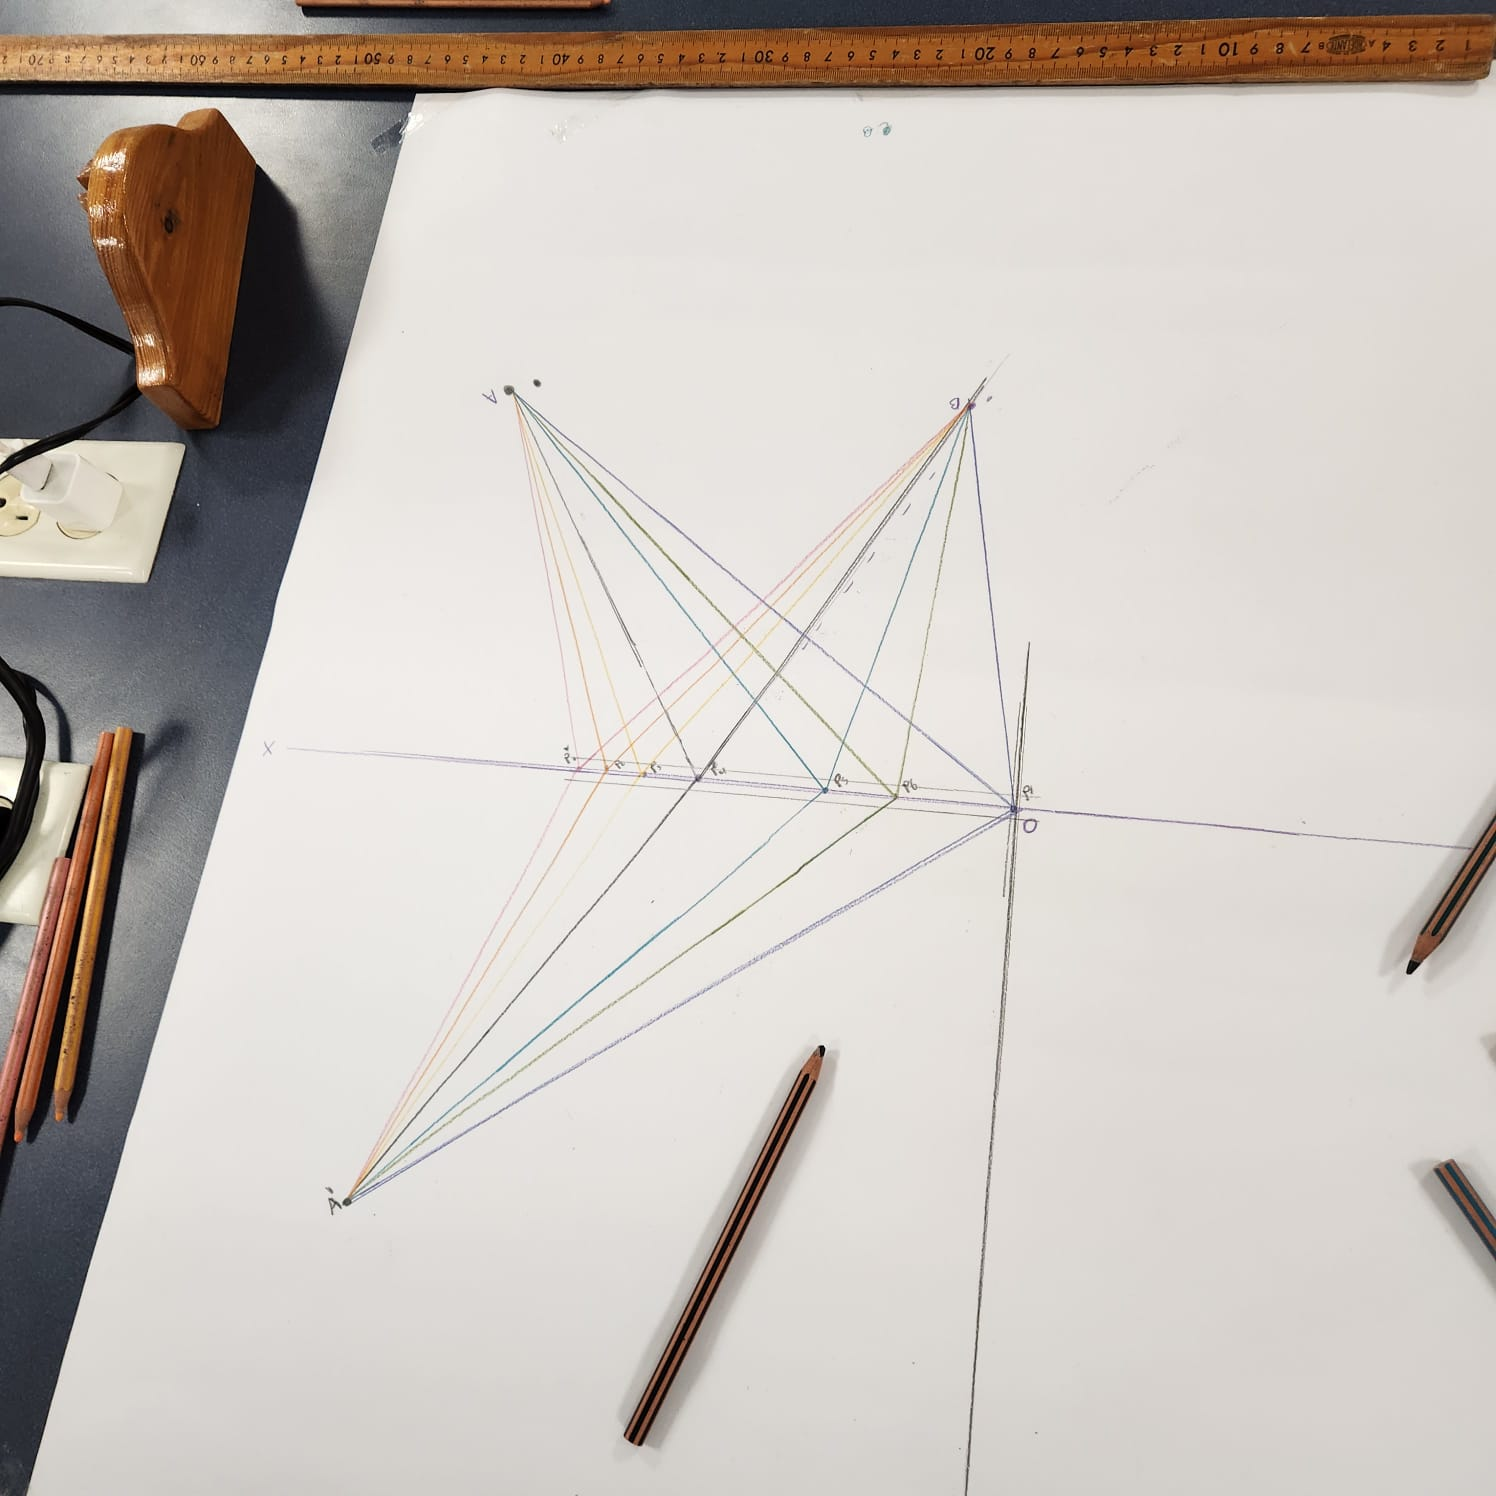
\includegraphics[width=\columnwidth]{trazo_fermat.jpg}
\captionof{figure}{Trazo de los siete caminos sobre el pliego. Arriba a la izquierda está el punto A, arriba a la derecha el punto B y abajo a la izquierda la imagen A'. Los puntos P1 a P7 están sobre la línea del espejo y O es el origen.}
\label{fig:trazo}
\end{center}

Con la regla medimos dos cosas para cada punto: su distancia horizontal $x$ al origen O y la longitud total del camino A', P, B, que según el marco teórico es igual a la del camino A, P, B. En la figura \ref{fig:girado} se muestra el mismo trazo visto desde otro ángulo, donde se aprecia mejor cómo todos los caminos de colores parten de A' y llegan a B.

\begin{center}
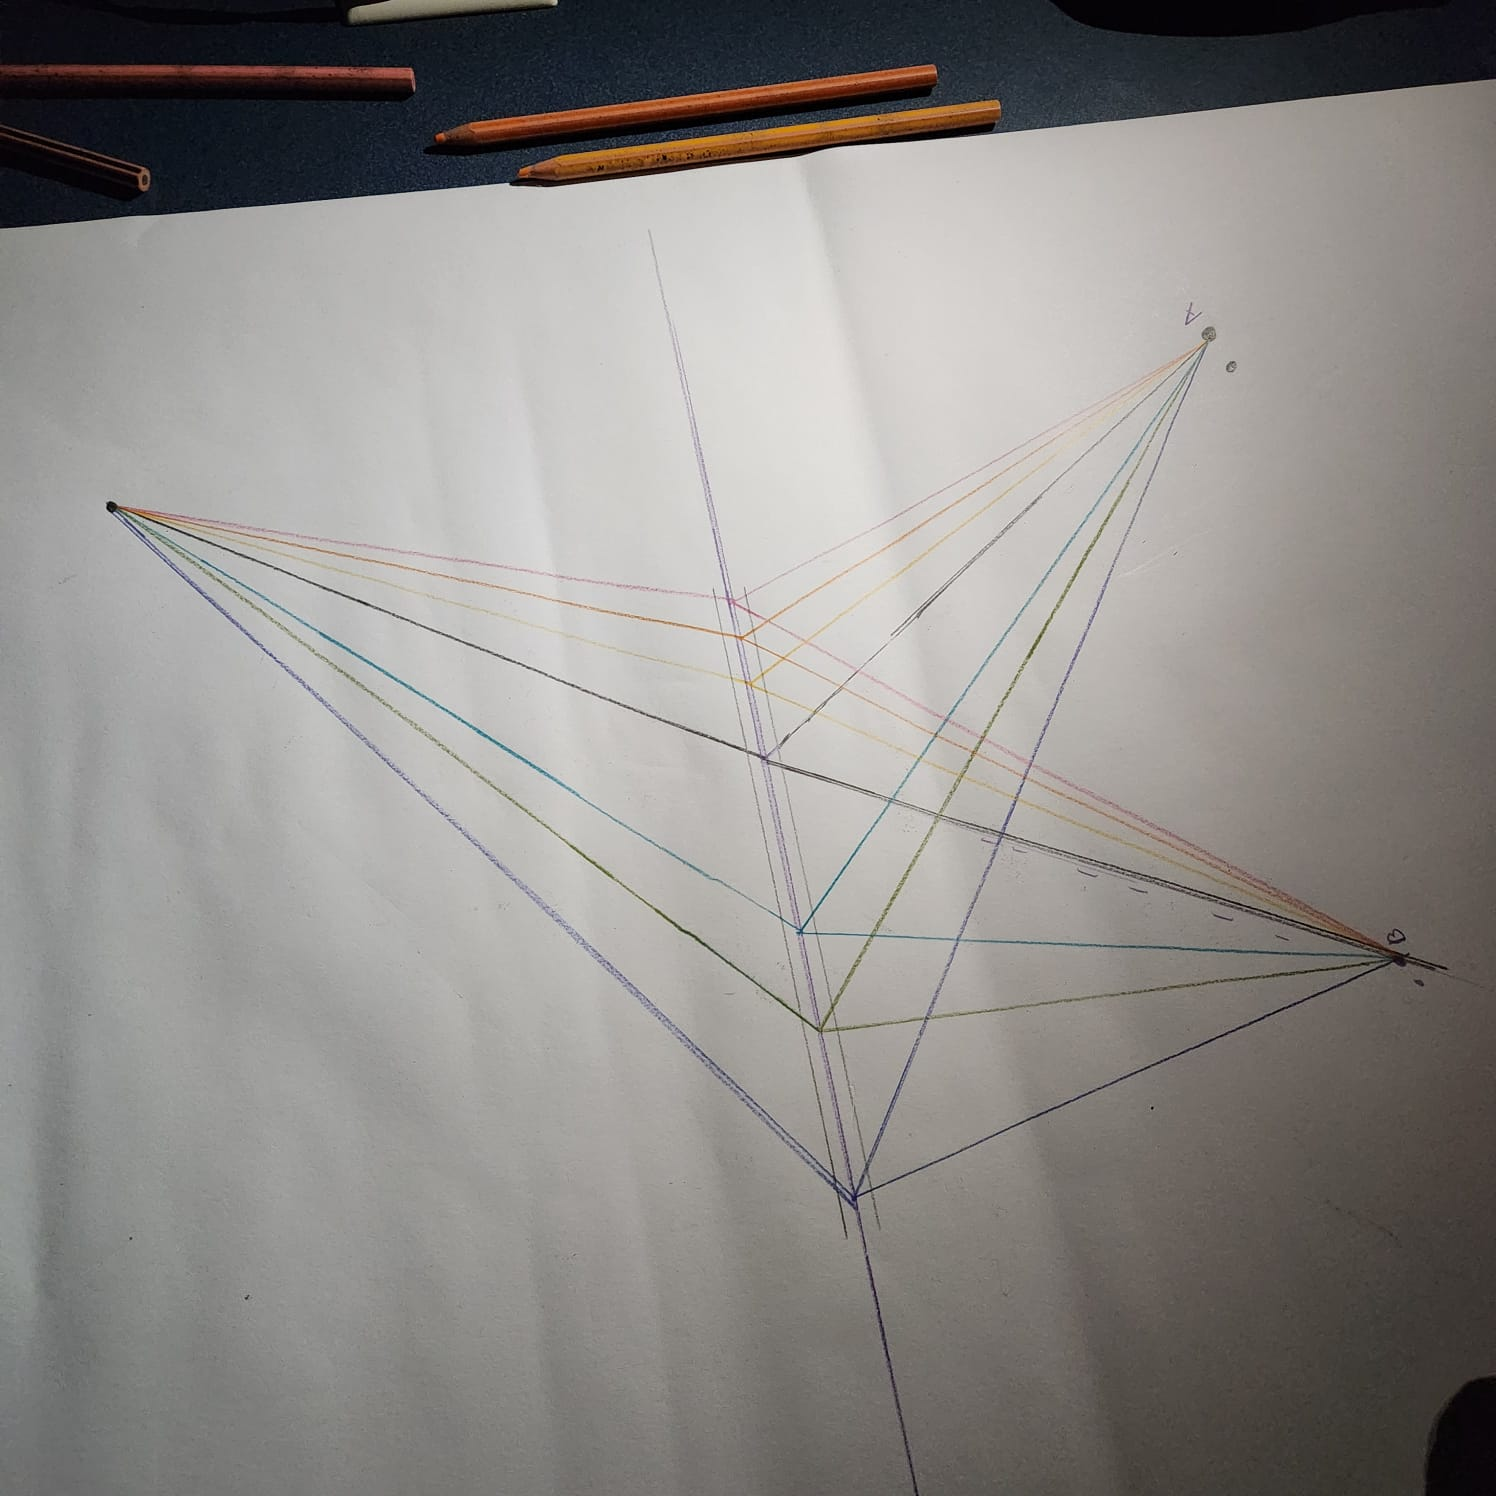
\includegraphics[width=\columnwidth]{trazo_fermat_girado.jpg}
\captionof{figure}{El mismo trazo girado, con el espejo en posición vertical. Los caminos de colores salen de A', tocan el espejo y terminan en B.}
\label{fig:girado}
\end{center}

Los valores se pasaron a una hoja de cálculo para graficar la longitud contra la distancia $x$ y buscar el punto más bajo de la curva.
